\label{sec-proofs}

This section is dedicated to the proofs of the
rearrangement theorem (\ref{thm-rearrange-weak}) and
the cancellation theorem (\ref{thm-cancel-weak})
for weak handlebodies.

\subsection{The rearrangement theorem}

\begin{definition}
    Let $M$ be a manifold.
    A smooth function $\theta\:M\to[0,1]$ is called a \term{level function},
    if $\theta^{-1}(0)=\partial M$ and $\theta$ has no critical points on $\partial M$.
\end{definition}

\begin{proposition}
    Every smooth manifold has a level function.
\end{proposition}

\begin{proof}
    Exercise for the reader.
\end{proof}

\begin{definition}
    Let $M$ be a manifold with a level function $\theta$, and let $\epsilon>0$.
    An \term{$\epsilon$-sliding} of $M$ is a diffeotopy $h\:M\times\R\to M$, such that
    \begin{enum}
        \item $h$ is supported in $\{p\in M\mid \theta(p)<\epsilon\}$.
        \item $\theta$ is preserved by $h$.
    \end{enum}
\end{definition}

Intuitively, an $\epsilon$-sliding moves the boundary around,
and keeps most of the interior fixed.
When we talk about an $\epsilon$-sliding,
we will implicitly assume that some level function $\theta$ is chosen.

\begin{lemma}\label{lem:slide}
Let $M$ be a manifold, and let $\epsilon>0$.
If $X$ is a compactly supported vector field on $\partial M$,
then $X$ can be extended to a vector field $\widetilde X$ on $M$,
which generates an $\epsilon$-sliding of $M$.
\end{lemma}

\begin{proof}
Let $U:=\{p\in M\mid \theta(p)<\epsilon\}$, 
where $\theta$ is the level function.
Let $K\subset\partial M$ denote the support of $X$.
Let $\partial M\times[0,+\infty)\subset M$ be a collar neighbourhood.
Since $K$ is compact,
we may assume $K\times[0,\epsilon]\subset U$.
We also assume that $\theta$ has no critical points in $K\times[0,\epsilon]$.

Let $\rho\:[0,+\infty)\to[0,1]$ be a smooth function such that
$\rho(0)=1$ and $\rho(r)=0$ when $r>\epsilon/2$.
We first extend $X$ to $M$ by letting
\[ X_p:=\biggl\{\mkern-3mu\begin{array}{ll}
\rho(r)\,X_q,&p=(q,r)\in K\times[0,\epsilon],\\
0,&\text{otherwise}.
\end{array} \]

Next we take a metric on $M$,
so that for all $p\in\partial M$, $\grad \theta(p)$ is orthogonal to $\T_p(\partial M)\subset\T_pM$.
This is possible by the constant rank theorem,
together with a partition of unity.
We define 
\[ \widetilde X:=X-\frac{\langle X,\grad \theta\rangle}{|\grad \theta|^2}\grad \theta. \]

Since $\widetilde X$ is supported in $K\times[0,\epsilon]$,
it generates a diffeotopy $h$.
Since $\widetilde X$ is orthogonal to $\grad\theta$,
$h$ is indeed an $\epsilon$-sliding. 
\end{proof}

\begin{remark}
If $X$ is instead supported in a disjoint union of countably many compact sets,
the lemma still holds true.
The reason is that the collar is global,
and will make sure that the sets $K\times[0,\epsilon]$ are disjoint.
\end{remark}

\begin{corollary}\label{cor:slide}
Every diffeotopy of $\partial M$ supported in
a disjoint union of compact sets 
can be extended to an $\epsilon$-sliding of $M$.
\end{corollary}

\begin{proof}
Apply (\ref{lem:slide}) to the velocity field of the diffeotopy.
This is a time-dependent vector field,
but the above proof applies as well.
\end{proof}

\begin{lemma}\label{lem:shrink}
    Let $(N,A)$ be a relative $n$-handlebody, 
    and let $\Phi\:\partial_1h^\lambda\to\partial N$ be an embedding,
    where $\lambda\neq0,n$.
    For any neighbourhood $U$ of the cobelt $\Phi(\partial D^\lambda\times0)$ in $\partial N$,
    the image of $\Phi$ can be moved into $U$ by an isotopy.
\end{lemma}
    
\begin{proof}
    Take any metric on $\partial N$.
    Then there exists $\epsilon>0$
    such that $\Phi(\partial D^\lambda\times\subsup D\epsilon{n-\lambda})\subset U$,
    where $\subsup D\epsilon{n-\lambda}$ denotes the disk of radius $\epsilon$.
    Now shrink $\Phi(\partial D^\lambda\times D^{n-\lambda})$ into this $\epsilon$-neighbourhood linearly.
\end{proof}

\begin{definition}
    Let $(N,A)$ be a weak relative $n$-handlebody, $i\geq0$ a fixed integer,
    and let $h\:N_i\to N_i$ be a diffeomorphism.
    The \term{perturbation by $h$} of $(N,A)$ is a relative handlebody $(N^h,A)$,
    with attaching maps $\Phi^h_j$, defined as follows:
    \begin{itms}
        \item $\subsup Njh=N_j$ and $\subsup\Phi jh=\Phi_j$ for all $j\leq i$.
        \item $\subsup\Phi{i+1}h=h\circ\Phi_{i+1}$. 
        This induces a diffeomorphism $h_{i+1}\:N_{i+1}\to\subsup N{i+1}h$.
        \item $\subsup\Phi{i+2}h=h_{i+1}\circ\Phi_{i+2}$,
        inducing a diffeomorphism $h_{i+2}\:N_{i+2}\to\subsup N{i+2}h$.
        \item And so on.
    \end{itms}
    The perturbation is called an \term{$\epsilon$-perturbation} if $h$ is an $\epsilon$-sliding.
    
    A finite composition of perturbations
    is also considered a perturbation.
\end{definition}

After a perturbation, the handles attached after the $i$-th step
will get attached to different handles,
but the new handlebody is similar to the original one.
We will see that every handlebody can be perturbed into a good one.

\begin{notation}
    Write
    \[ \partial_1h^\lambda := \partial D^\lambda \times D^{n-\lambda}
    \quad\text{and}\quad
    \partial_2h^\lambda := D^\lambda \times \partial D^{n-\lambda}, \]
    so that $\partial h^\lambda = \partial_1h^\lambda \cup \partial_2h^\lambda$.
    \varqed
\end{notation}

The idea of our proof of the rearrangement theorem 
is to create a vector field on the side of each handle,
so that other handles attached on it
can be slid out of it along this vector field.

\begin{definition}
    Let $h^\lambda$ be a $\lambda$-handle, where $\lambda\neq0,n$.
    Let $B\subset\partial_2h^\lambda$ be a closed subset,
    and let $O$ denote the belt of $h^\lambda$.
    An \term{expanding field} of $h^\lambda$ with respect to $B$
    is a vector field $X$ on $\partial_2h^\lambda$, such that
    \begin{itms}
        \item $X_p=0$ if and only if $p\in B\cup O$.
        %\item $X_p$ points outwards for $p\in\partial(\partial_2h^\lambda)-B$.
        \item For every $p\in\partial_2h^\lambda\setminus(B\cup O)$,
        the flow line of $X$ starting from $p$ reaches $\partial\partial_2h^\lambda$ within finite time.
    \end{itms}
    
    Let $(N,A)$ be a finite relative $n$-handlebody.
    Its \term{skeleton} is defined to be the set $\Sigma$ of compact submanifolds of $\partial N$,
    consisting of
    \begin{enum}
        \item The intersection of $\partial N$ with
        the boundary of the image of every attaching map.
        \item The intersection of $\partial N$ with
        the belt of each handle.
        \item All possible intersections of the manifolds listed above.
    \end{enum}
    In order for \textup{(iii)} to be well-defined, we require that
    the set of submanifolds in \textup{(i)} and \textup{(ii)} is transverse.
    Such a finite relative handlebody is said to be \term{regular}.
    We denote by $\Sigma_i$ the skeleton of $(N_i,A)$,
    and call it the \term{$i$-skeleton} of $(N,A)$.
    
    A regular $n$-handlebody $(N,A)$ is said to be \term{expanded},
    if every $\lambda$-handle $h^\lambda$ with $\lambda\neq0,n$ has an expanding field
    with respect to the union of images of attaching maps of handles
    that are attached after it.
\end{definition}

An expanding field does not necessarily exist for arbitrary $B$.
For example, consider the case $n=2$, $\lambda=1$ and $B$ is a point not in $O$.

The next lemma makes clear how expanding fields work.
The main idea of the proof is visualised below.
\[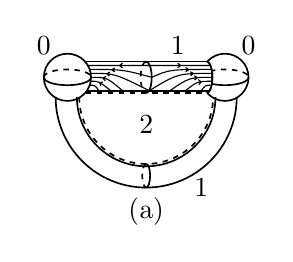
\begin{tikzpicture}[line width=.6, baseline=(base.base)]
    \tikzstyle{dp}=[dash pattern=on 2pt off 2pt]
    \draw (-1,0) circle (0.3);
    \draw (1,0) circle (0.3);
    \draw[dp] (-1.3,0) arc (180:0:0.3 and 0.1);
    \draw (-1.3,0) arc (180:360:0.3 and 0.1);
    \draw[dp] (.7,0) arc (180:0:0.3 and 0.1);
    \draw (.7,0) arc (180:360:0.3 and 0.1);
    \draw[dp,fill=white] (.77,0) ellipse (.07 and .2);
    \fill[white] (.72,0) ellipse (.07 and .2);
    \draw (-.77,.2) -- (.77,.2);
    \draw[dp] (-.77,-.2) -- (.77,-.2);
    \draw (-.75,-.17) -- (.8,-.17);
    \draw (.77,.2) arc (90:-90:.07 and .2);
    \draw (0,.2) arc (90:-90:.07 and .2);
    \draw[dp] (0,.2) arc (90:270:.07 and .2);
    \draw (-1.15,-.25) arc (180:360:1.15);
    \draw[dp] (-.85,-.25) arc (180:360:.85);
    \draw (-.88,-.25) arc (180:360:.88);
    \draw (0,-1.1) arc (90:-90:.05 and .15);
    \draw[dp] (0,-1.1) arc (90:270:.05 and .15);

    \draw[thin] (0,.15) -- (.82,.15) (.4,.18) -- (.44,.15) -- (.4,.12); 
    \draw[thin] (.07,0) .. controls (.3,.1) and (.3,.1) .. (.84,.1) (.5,.125) -- (.54,.095) -- (.5,.07);
    \draw[thin] (.04,-.17) .. controls (.4,.05) and (.4,.05) .. (.85,.05) (.56,.07) -- (.6,.05) -- (.565,.02);
    \draw[thin] (.3,-.17) .. controls (.55,0) and (.55,0) .. (.85,0) (.61,.02) -- (.65,-.005) -- (.615,-.035);
    \draw[thin] (.5,-.17) .. controls (.65,-.05) and (.65,-.05) .. (.85,-.05) (.66,-.03) -- (.7,-.057) -- (.67,-.095);
    \draw[thin] (.7,-.17) .. controls (.75,-.1) and (.75,-.1) .. (.84,-.1);
    
    \draw[thin] (.04,.15) -- (-.74,.15) (-.3,.18) -- (-.34,.15) -- (-.3,.12); 
    \draw[thin] (.07,0) .. controls (-.3,.1) and (-.3,.1) .. (-.72,.1) (-.4,.12) -- (-.44,.095) -- (-.4,.07);
    \draw[thin] (.04,-.17) .. controls (-.4,.05) and (-.4,.05) .. (-.7,.05) (-.46,.067) -- (-.5,.045) -- (-.465,.015);
    \draw[thin] (-.3,-.17) .. controls (-.5,0) and (-.5,0) .. (-.7,0) (-.51,.012) -- (-.55,-.008) -- (-.52,-.045);
    \draw[thin] (-.45,-.17) .. controls (-.6,-.05) and (-.6,-.05) .. (-.7,-.05) (-.55,-.06) -- (-.59,-.07) -- (-.575,-.11);
    \draw[thin] (-.6,-.17) .. controls (-.65,-.1) and (-.65,-.1) .. (-.72,-.1);

    \node at (0,-0.6) {2};
    \node at (.4,0.4) {1};
    \node at (.7,-1.4) {1};
    \node at (1.3,0.4) {0};
    \node at (-1.3,0.4) {0};
    \node (base) at (0,-1.7) {(a)};
\end{tikzpicture}
\qquad
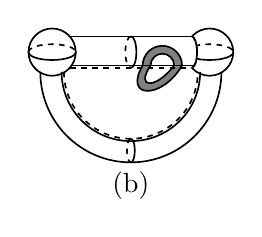
\begin{tikzpicture}[line width=.6, baseline=(base.base)]
    \tikzstyle{dp}=[dash pattern=on 2pt off 2pt]
    \fill[black!50] (.15,-.17) arc (180:0:.25);
    \fill[white] (.25,-.17) arc (180:0:.15);
    \fill[black!50] (.15,-.17) .. controls (-.1,-.6) and (.4,-.6) .. (.65,-.17);
    \fill[white] (.25,-.17) .. controls (.05,-.47) and (.32,-.47) .. (.55,-.17);
    \draw (-1,0) circle (0.3);
    \draw (1,0) circle (0.3);
    \draw[dp] (-1.3,0) arc (180:0:0.3 and 0.1);
    \draw (-1.3,0) arc (180:360:0.3 and 0.1);
    \draw[dp] (.7,0) arc (180:0:0.3 and 0.1);
    \draw (.7,0) arc (180:360:0.3 and 0.1);
    \draw[dp,fill=white] (.77,0) ellipse (.07 and .2);
    \fill[white] (.72,0) ellipse (.07 and .2);
    \draw (-.77,.2) -- (.77,.2);
    \draw[dp] (-.77,-.2) -- (.77,-.2);
    \draw (-.75,-.17) -- (.8,-.17);
    \draw (.77,.2) arc (90:-90:.07 and .2);
    \draw (0,.2) arc (90:-90:.07 and .2);
    \draw[dp] (0,.2) arc (90:270:.07 and .2);
    \draw (-1.15,-.25) arc (180:360:1.15);
    \draw[dp] (-.85,-.25) arc (180:360:.85);
    \draw (-.88,-.25) arc (180:360:.88);
    \draw (0,-1.1) arc (90:-90:.05 and .15);
    \draw[dp] (0,-1.1) arc (90:270:.05 and .15);
    \draw (.15,-.17) arc (180:0:.25);
    \draw (.25,-.17) arc (180:0:.15);
    \draw (.15,-.17) .. controls (-.1,-.6) and (.4,-.6) .. (.65,-.17);
    \draw (.25,-.17) .. controls (.05,-.47) and (.32,-.47) .. (.55,-.17);
    \node (base) at (0,-1.7) {(b)};
\end{tikzpicture}
\qquad
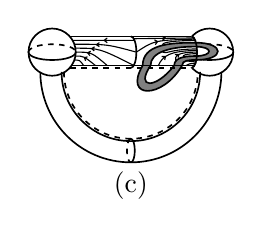
\begin{tikzpicture}[line width=.6, baseline=(base.base)]
    \tikzstyle{dp}=[dash pattern=on 2pt off 2pt]
    \draw (-1,0) circle (0.3);
    \draw (1,0) circle (0.3);
    \draw[dp] (-1.3,0) arc (180:0:0.3 and 0.1);
    \draw (-1.3,0) arc (180:360:0.3 and 0.1);
    \draw[dp] (.7,0) arc (180:0:0.3 and 0.1);
    \draw (.7,0) arc (180:360:0.3 and 0.1);
    \draw[dp,fill=white] (.77,0) ellipse (.07 and .2);
    \fill[white] (.72,0) ellipse (.07 and .2);
    \fill[black!50] (.15,-.17) .. controls (-.1,-.6) and (.4,-.6) .. (.65,-.17);
    \fill[white] (.25,-.17) .. controls (.05,-.47) and (.32,-.47) .. (.55,-.17);
    \fill[black!50] (.15,-.17) .. controls (.15,.1) and (.5,.12) .. (.82,.12)
    				 .. controls (1.2,.12) and (1.2,-.1) .. (.82,-.1)
    				 .. controls (.75,-.1) and (.65,-.1) .. (.65,-.17);
    \fill[white] (.25,-.17) .. controls (.25,0) and (.5,.07) .. (.82,.07)
    				 .. controls (1.05,.07) and (1.05,-.05) .. (.82,-.05)
    				 .. controls (.75,-.05) and (.55,-.05) .. (.55,-.17); 
    \draw (-.77,.2) -- (.77,.2);
    \draw[dp] (-.77,-.2) -- (.77,-.2);
    \draw (-.75,-.17) -- (.8,-.17);
    \draw (.77,.2) arc (90:-90:.07 and .2);
    \draw (0,.2) arc (90:-90:.07 and .2);
    \draw (-1.15,-.25) arc (180:360:1.15);
    \draw[dp] (-.85,-.25) arc (180:360:.85);
    \draw (-.88,-.25) arc (180:360:.88);
    \draw (0,-1.1) arc (90:-90:.05 and .15);
    \draw[dp] (0,-1.1) arc (90:270:.05 and .15);
    \draw (.15,-.17) .. controls (-.1,-.6) and (.4,-.6) .. (.65,-.17);
    \draw (.25,-.17) .. controls (.05,-.47) and (.32,-.47) .. (.55,-.17);
    \draw (.15,-.17) .. controls (.15,.1) and (.5,.12) .. (.82,.12)
    				 .. controls (1.2,.12) and (1.2,-.1) .. (.82,-.1)
    				 .. controls (.75,-.1) and (.65,-.1) .. (.65,-.17);
    \draw (.25,-.17) .. controls (.25,0) and (.5,.07) .. (.82,.07)
    				 .. controls (1.05,.07) and (1.05,-.05) .. (.82,-.05)
    				 .. controls (.75,-.05) and (.55,-.05) .. (.55,-.17); 
	\draw[thin] (.04,.15) -- (-.74,.15) (-.3,.18) -- (-.34,.15) -- (-.3,.12); 
    \draw[thin] (.07,0) .. controls (-.3,.1) and (-.3,.1) .. (-.72,.1) (-.4,.12) -- (-.44,.095) -- (-.4,.07);
    \draw[thin] (.04,-.17) .. controls (-.4,.05) and (-.4,.05) .. (-.7,.05) (-.46,.067) -- (-.5,.045) -- (-.465,.015);
    \draw[thin] (-.3,-.17) .. controls (-.5,0) and (-.5,0) .. (-.7,0) (-.51,.012) -- (-.55,-.008) -- (-.52,-.045);
    \draw[thin] (-.45,-.17) .. controls (-.6,-.05) and (-.6,-.05) .. (-.7,-.05) (-.55,-.06) -- (-.59,-.07) -- (-.575,-.11);
    \draw[thin] (-.6,-.17) .. controls (-.65,-.1) and (-.65,-.1) .. (-.72,-.1);

	\draw[thin] (.03,.17) -- (.8,.18) (.4,.2) -- (.44,.18) -- (.4,.15); 
	\draw[thin] (.07,0) .. controls (.3,.15) and (.3,.15) .. (.8,.165) (.3,.155) -- (.34,.135) -- (.31,.095);
	\draw[thin] (.4,.08) .. controls (.4,.11) and (.4,.14) .. (.82,.15);
	\draw[thin] (.4,0) .. controls (.45,-.03) and (.5,.04) .. (.84,.04);
	\draw[thin] (.35,-.17) .. controls (.4,-.05) and (.5,.02) .. (.84,.02) (.39,-.055) -- (.44,-.055) -- (.43,-.1);
	\draw[thin] (.57,-.12) .. controls (.55,-.04) and (.6,.0) .. (.84,.0) (.56,-.03) -- (.61,-.03) -- (.6,-.07);
	\draw[thin] (.67,-.06) .. controls (.65,-.04) and (.7,-.02) .. (.84,-.02);
	
	\draw[thin] (.7,-.11) .. controls (.75,-.125) and (.75,-.125) .. (.82,-.125);
    \draw[thin] (.7,-.17) .. controls (.75,-.145) and (.75,-.145) .. (.82,-.145);
    \node (base) at (0,-1.7) {(c)};
\end{tikzpicture}\]

\begin{center}
    \parbox{96mm}{\small\leftskip=1.5em\parindent=-1.5em
    (a) A $4$-handlebody, where numbers indicate types of handles.
    A $1$-handle is drawn with its expanding field.
    (Of course what is seen here is a $3$-dimensional analogue of the real thing.)
    
    (b) Attach a $3$-handle,
    where the shaded part indicates the image of the attaching map.
    
    (c) Stretch the attaching map using the expanding field,
    and construct a new expanding field on the $1$-handle.}\vspace{1pt}
\end{center}

\begin{lemma}\label{lem:expanded}
    Let $(N,A)$ be a finite relative $n$-handlebody with $i$ handles,
    such that $(N_{i-1},A)$ is good and expanded.
    Then $N_{i-1}$ can be $\epsilon$-slid,
    so that the induced $\epsilon$-perturbation is good and expanded.
\end{lemma}
    
\begin{proof}
    Let $h^\lambda$ denote the handle to be attached,
    and let $\Phi$ denote the attaching map.
    Let $h_j$ denote the handle attached in the $j$-th step.
    Since $(N_{i-1},A)$ is good, we may assume $h_1,\dotsc,h_{i-1}$ are of ascending types.
    
    First we try to slide $\image(\Phi)$ to avoid all handles of type $\geq\lambda$.
    Suppose $\image(\Phi)$ intersects with some $h_{\smash{j}}$ with type $\geq\lambda$,
    and we fix the largest $j$ with this property.
    Then $\image(\Phi)$ does not intersect with $h_{\smash{j+1}},\dotsc,h_{i-1}$.
    By reparametrising $h^\lambda$,
    we may assume that the cobelt $\Phi(\partial D^\lambda\times0)$ avoids the belt $O$ of $h_j$.
    By (\ref{lem:shrink}), we can shrink $\image(\Phi)$
    so that it does not meet $O$.
    We then extend the expanding field on $h_j$ to a small neighbourhood
    in $\partial N_j\cap\partial N_{i-1}$
    that does not meet any handles attached after the $j$-th step,
    and we could slide $\image(\Phi)$ out of $\partial_2h_j$
    using the flow $\phi_t$ of the expanding field for large enough $t$.
    We do this for all $h_j$, in descending order
    until $\image(\Phi)$ finally gets to a (literally) good position,
    i.e.\ within $\partial N_{i'-1}$, where
    $i'$ denotes the step where the first handle of type $\geq\lambda$ is attached.
    
    Our next plan is to do an $\epsilon$-sliding for each $j=i'-1,\dotsc,1$,
    making the corresponding handle expanded at each time.
    By (\ref{cor:transverse}), we may assume that
    $\Phi(\partial\partial_2h^{\lambda})$ is transverse to
    everything in $\Sigma_{i'-1}$,
    while keeping $\image(\Phi)$ disjoint with $h_{i'},\dotsc,h_{i-1}$.
    
    In the $j$-th step,
    let $X$ denote the expanding field on $\partial_2h_j$.
    Let $B\subset\partial N_j$ denote the union of images of attaching maps in steps $j+1,\dotsc,i-1$,
    intersected with $\partial N_j$.
    Let $\Phi'$ denote the composition of $\Phi$ with the previously executed slidings.
    
    Let $S_{j+1},\dotsc,S_i$
    be the boundaries of images of attaching maps
    in the corresponding steps, intersected with $\partial N_j$,
    so that $S_i=\Phi'(\partial\partial_2h^{\smash{\lambda}})\cap\partial N_j$.
    Let $O$ denote the belt of $h_j$.
    Thus the $S_k$ and $B$ are submanifolds possibly with corners,
    and the corners of $B$ are concave.
    By (\ref{lem:extension}) and the remark after it,
    we may extend the $S_k$ that have boundaries a little bit into $B$,
    so that the extended manifolds $\subsup Sk\prime$ are compact,
    and $\partial\subsup Sk\prime\subset B^\circ$ for all $k$.
    %(This can be achieved, for example, by projecting a compact collar of
    %$\partial\partial_2h_k$ in $\partial_2h_k$
    %to a collar of $\partial\partial_2h_k$ in $\partial N_{k-1}$ diffeomorphically,
    %and then projecting it to $\partial N_{k-2},\dotsc,$ and finally to $\partial N_j$.)
    
    By regularity of $(N_{i-1},A)$,
    we may assume $O,\subsup S{j+1}\prime,\dotsc,\subsup Si\prime$ are transverse
    (shrinking a bit the extended part if necessary).
    Thus by (\ref{cor:function}),
    there is a smooth function $f\:\partial N_j\setminus B^\circ\to[0,1]$,
    with $f^{\smash{-1}}(0)=(O\cup\subsup S{j+1}\prime\cup\cdots\cup\subsup Si\prime)\setminus B^\circ$,
    with no critical values other than $0,1$.
    We modify $f$ by letting $f|_B\equiv0$ and $f|_{\image(\Phi')}\equiv0$.
    Now $f$ becomes a smooth function $\partial N_j\to[0,1]$ with $f^{-1}(0)=O\cup B\cup\image(\Phi')$,
    and it has no critical values other than $0,1$.

    We extend $X$ to a compactly supported smooth vector field on $\partial N_j$,
    so that $X|_{B}=0$, and for any $p\in\partial\partial_2h_j$ such that $X_p\neq0$,
    the change of $f$ along the extended part of the flow line of $X$ through $p$ is $<1/2$.
    
    %Notice that any vector field $X'$ that is
    %close enough to $X$ in the sense of (\ref{lem:transversal})
    %is an expanding field.
    %Thus by (\ref{lem:transversal}), we may take such an expanding field $X'$,
    We take a large number $t\in\R$,
    such that the flow $h:=\phi_t$ of $X$ satisfies
    \[h\bigl(f^{-1}([1/2,1])\cap\partial_2h_j\bigr)\cap\partial_2h_j=\emptyset.\]
    By (\ref{cor:transverse}), after performing a small isotopy
    preserving the above condition, keeping $B$ fixed,
    we may assume that $h(\Phi'(\partial\partial_2h^\lambda))$ is transverse to
    everything in $\Sigma_{i-1}$.
    
    Take a metric on $\partial_2h_j$, and put
    \[ Y_p:=\d h(\grad f(h^{-1}(p))). \]
    One verifies that $Y$ is a new expanding field on $\partial_2h_j$, 
    but with respect to $B\cup\image(h\circ\Phi')$ instead of $B$.
    Note that $h$ keeps $B$ fixed.
    Finally we execute the $\epsilon$-sliding induced by $h$.
    
    We have finished the $j$-th step.
    Running over $j=i'-1,\dotsc,1$ gives a desired $\epsilon$-sliding,
    and gives desired expanding fields on all handles except the $i$-th one.
    But the $i$-th handle is trivially done.
    Regularity is preserved throughout the above construction.
\end{proof}

Having done much preparatory work,
we are finally ready to take our final step to proving (\ref{thm-rearrange-weak}),
namely, the concatenation of these infinitely many slidings
given by the preceding lemma.

\begin{proof}[Proof of \textup{(\ref{thm-rearrange-weak})}]
Let $(N,A)$ be a weak relative $n$-handlebody.
We may assume that only one handle is attached in each step.
For each $i\geq0$, we may regard $(N_i,A)$ as a non-weak relative handlebody.
Let $\theta_i$ be a level function on $N_i$ for $i=0,1,\dotsc$,
so that $\theta_i\leq\theta_{i+1}$ for all $i$.
%Denote $\subsup Ni\circ=N_i-\partial N_i$,
%and denote $\Theta(p):=\theta_i(p)$ if $p\in\subsup Ni\circ-\subsup N{i-1}\circ$,
%where $\subsup N{-1}\circ$ is understood to be the empty set.
%Thus $\Theta$ is a function 

Denote $N^1=N$. Note that $(\subsup N11,A)$ is automatically expanded.
By (\ref{lem:expanded}),
$\subsup N11$ can be $1/2$-slid,
so that if we denote by $(N^2,A)$ the induced perturbation,
then $(\subsup N22,A)$ is expanded. 
We continue to $1/4$-slide $\subsup N22$ to get a perturbation $(N^3,A)$ of $(N^2,A)$,
so that $(\subsup N33,A)$ is expanded.
Continuing this process, using $1/2^i$ in the $i$-th step,
we get a commutative grid of maps
\[ \begin{tikzcd}
\subsup N01\ar[r,hook] &\subsup N11\ar[r,hook]\ar[d,"\simeq"] &\subsup N21\ar[r,hook]\ar[d,"\simeq"] &\subsup N31\ar[r,hook]\ar[d,"\simeq"] &\subsup N41\ar[r,hook]\ar[d,"\simeq"] &\cdots\\
\subsup N02\ar[r,hook] &\subsup N12\ar[r,hook] &\subsup N22\ar[r,hook]\ar[d,"\simeq"] &\subsup N32\ar[r,hook]\ar[d,"\simeq"] &\subsup N42\ar[r,hook]\ar[d,"\simeq"] &\cdots\\
\subsup N03\ar[r,hook] &\subsup N13\ar[r,hook] &\subsup N23\ar[r,hook] &\subsup N33\ar[r,hook]\ar[d,"\simeq"] &\subsup N43\ar[r,hook]\ar[d,"\simeq"] &\cdots\rlap,\\
&&&\dots&\dots
\end{tikzcd} \]
where the vertical maps are all diffeomorphisms.
By construction $\subsup Nii$ and $\subsup Ni{i+1}$ are naturally identified,
but note that the identification is not the diffeomorphism (sliding) in the diagram.
We define $\theta_i$ on $\subsup N{\smash{j}}i$ for $i\leq j+1$ to be the
level function inherited from $N_j=\subsup Nj1$.
Thus for $\subsup Nii$ and $\subsup Ni{i+1}$,
their functions $\theta_i$ are the same under the natural identification.

We define a good weak relative $n$-handlebody $(N',A)$ 
by $\subsup Ni\prime:=\subsup Nii$, 
and the inclusion maps being $\subsup Nii=\subsup Ni{i+1}\hookrightarrow\subsup N{i+1}{i+1}$.
This is \emph{not} the map in the above diagram!
But for $p\in\subsup Nii\subset\subsup N{i+1}{i+1}$, we still have
$\theta_i(p)\leq\theta_{i+1}(p)$.
We will show that $N$ is diffeomorphic to $N'$. 

Consider the (not commutative) diagram
\[ \begin{tikzcd}
N_1\ar[d,equals]\ar[r,hook] &N_2\ar[d,"\simeq"]\ar[r,hook] &N_3\ar[d,"\simeq"]\ar[r,hook] &\cdots\\
\subsup N11\ar[r,hook] &\subsup N22\ar[r,hook] &\subsup N33\ar[r,hook] &\cdots\rlap,
\end{tikzcd}\eqno(*) \]
where the vertical maps are as in the above grid-like diagram.
By comparing the above two diagrams, the square
\[ \begin{tikzcd}
N_i\ar[r,hook]\ar[d,"\simeq"] &N_{i+1}\ar[d,"\simeq"]\\
\subsup Nii\ar[r,hook] &\subsup N{i+1}{i+1}
\end{tikzcd} \]
commutes for some $p\in N_i$
if and only if $p$ is fixed by the sliding $\subsup Nii\to\subsup Ni{i+1}$.
This happens whenever $\theta_i(p)>1/2^i$. Thus for
\[ U_i:=\{p\in N_i\mid\theta_i(p)>1/2^i\}, \]
the diagram $(*)$ commutes after the $i$-th square.
Thus we have an induced diffeomorphism of $U_i$ onto a subset of $N'$.
Since $N=\bigcup_{i=1}^\infty U_i$, we have an induced map $\phi\:N\to N'$
which is a diffeomorphism onto its image.
Clearly $\phi$ is also surjective since $N'=\bigcup_{i=1}^\infty\image(U_i\to N')$.
Thus $\phi$ is a diffeomorphism. 
\end{proof}

\subsection{The cancellation theorem}

We first state the cancellation theorem
for finite handlebodies.

\begin{theorem}[Cancellation, finite case]\label{thm:cancel}
Let $N=A\cup_{\Phi_1}h^\lambda\cup_{\Phi_2}h^{\lambda+1}$ be a relative handlebody with $2$ handles.
If the cobelt of $h^{\lambda+1}$ and the belt of $h^\lambda$ intersect transversely
at precisely one point, then $N$ is diffeomorphic to $A$.
This diffeomorphism can be taken to be fixed on any closed subset of $A\setminus\image(\Phi_1)\setminus\image(\Phi_2)$.
\end{theorem}

\begin{proof}
\cite[Theorem~5.4.3]{wall} or \cite[Theorem~3.34]{matsu}.
\end{proof}

For convenience, we introduce the following terminology.
In a good relative handlebody, a pair of $\lambda$- and $(\lambda+1)$-handles is called a
\term{cancelling pair}, if the cobelt of the $(\lambda+1)$-handle
and the belt of the $\lambda$-handle intersect transversely
at precisely one point. 
The $(\lambda+1)$-handle will be called the \term{canceller},
and the $\lambda$-handle will be called the \term{cancellee}.

We say that we can \term{cancel} a set $S$ of handles from a weak relative handlebody $(N,A)$,
if $N$ is diffeomorphic to a weak relative handlebody,
whose $\lambda$-handles correspond to
the $\lambda$-handles of $N$ that are not in $S$,
and the combinatorics concerning which handles are attached to other handles should not change,
except that a handle attached to a cancelled handle may get attached to
a handle which a cancelled handle was attached to.

\begin{theorem}[Cancellation, infinite case] \label{thm:cancel-infinite}
Let $(N,A)$ be a weak relative handlebody whose handles are attached one at a time,
and let $S$ be a set of handles consisting of cancelling pairs
that do not have handles in common,
such that every canceller in $S$ is attached immediately after its cancellee.
Then $S$ can be cancelled.
\end{theorem}

\begin{proof}
We will construct a new weak handlebody $N'$ diffeomorphic to $N$,
with the desired property.

Let $\subsup N0\prime:=N_0=A$, and let $\theta_0$ be a level function on it.
Let $\phi_0\:N_0\to\subsup N0\prime$ be a diffeomorphism.
As we construct $N'$, we will construct diffeomorphisms $\phi_i\:N_i\to\subsup Ni\prime$,
and level functions $\theta_i$ on $\subsup Ni\prime$,
such that $\theta_i\leq\theta_{i+1}$ on $\subsup Ni\prime$.
This will be implicit in the below construction.

In the $i$-th step, if the $i$-th handle of $N$ is not a canceller or a cancellee,
then we attach a same handle to $N'$ according to $\phi_{i-1}$,
and let $\phi_i$ be the induced diffeomorphism.
If it is a cancellee (followed by its canceller),
then we will not attach handles to $N'$ in the $i$-th and $(i+1)$-th steps.
Instead, we construct by (\ref{thm:cancel}) a diffeomorphism $\phi_{i+1}$ to form a (not commutative) diagram
\[ \begin{tikzcd}
N_{i-1}\ar[d,"\phi_{i-1}"',"\simeq"]\ar[r,hook] &N_i\ar[r,hook] &N_{i+1}\ar[d,"\phi_{i+1}"',"\simeq"]\\
\subsup N{i-1}\prime\ar[r,equals] &\subsup Ni\prime\ar[r,equals] &\subsup N{i+1}\prime\rlap.
\end{tikzcd} \]
By the last statement of (\ref{thm:cancel}), we may require the diagram to commute in
$\subsup U{i-1}\prime:=\{p\in\subsup N{i-1}\prime\mid\theta_{i-1}(p)>1/2^{i-1}\}$.
We take a new level function $\theta_{i+1}$ on $\subsup N{i+1}\prime$,
so that for all $p\in\subsup N{i-1}\prime$, we have
\[\theta_{i+1}(p)\geq\theta_{i-1}(p)\quad\text{and}\quad
\theta_{i+1}(p)\geq\theta_{i-1}(\phi_{i+1}\circ\subsup{\phi}{i-1}{-1}(p)).\]
By a same argument as before, we have a colimit map from $N'$ to $N$,
which is an embedding. It is surjective by the choice of the functions $\theta_i$.
\end{proof}

We have now completed the proof of our two 
main theorems. They can be combined to obtain
the following result, which simplifies weak handlebodies.

\begin{definition}
Let $n\geq m\geq0$ be integers. An \term{$(n,m)$-handlebody} is an $n$-handlebody
whose handles are of type $0,1,\dotsc,m$.
\end{definition}

\begin{corollary}\label{prop:0-handle}
Every connected finite handlebody is diffeomorphic to
a handlebody with only one $0$-handle.
Every connected weak handlebody is diffeomorphic to
a good weak handlebody with only one $0$-handle.
\end{corollary}

\begin{proof}
For the finite case, we may suppose that the handlebody is good by (\ref{thm-rearrangement}).
Thus it suffices to prove the statement for an $(n,1)$-handlebody.
Consider a graph with vertices corresponding to the $0$-handles
and edges corresponding to the $1$-handles.
Then this graph is connected.
Taking a maximal tree of this graph,
we may assume the handlebody is simply connected
(by discarding the $1$-handles not in the tree).
Thus the result follows from (\ref{thm:cancel}),
by cancelling the $0$- and $1$-handles a pair at a time.

For the weak case, we suppose that the handlebody is good by (\ref{thm-rearrange-weak}).
We construct a graph and take a maximal tree in the same way,
and the statement follows from (\ref{thm:cancel-infinite}).
\end{proof}
